\documentclass[12pt,a4paper]{article}
\usepackage[utf8]{inputenc}
\usepackage[english]{babel}
\usepackage{graphicx}
\usepackage{listings}
\usepackage{xcolor}
\usepackage{tikz}
\usetikzlibrary{arrows,positioning,shapes.geometric,shapes.multipart}
\usepackage{geometry}
\geometry{margin=1in}

% Code listing settings
\lstset{
    language=Python,
    basicstyle=\ttfamily\small,
    keywordstyle=\color{blue},
    commentstyle=\color{green!50!black},
    stringstyle=\color{red},
    numbers=left,
    numberstyle=\tiny\color{gray},
    stepnumber=1,
    numbersep=5pt,
    backgroundcolor=\color{gray!10},
    frame=single,
    breaklines=true,
    captionpos=b
}

\title{\textbf{Practice 3: MPI File Transfer System}  \\ 
       \large Distributed Systems Course}
\author{Nguyen Tien Duy \\ Student ID: 22BA13102}
\date{}

\begin{document}

\maketitle

\section{Introduction}

This report describes the implementation of a file transfer system using MPI (Message Passing Interface). This work builds upon the TCP-based file transfer system from Practice 1, upgrading it to use MPI for inter-process communication in distributed computing environments.

Unlike the client-server architecture of TCP sockets, MPI uses a process-based model where all processes start simultaneously and communicate through message passing. This approach is particularly suited for high-performance computing (HPC) environments and parallel applications.

\section{Why mpi4py?}

For this implementation, I chose \textbf{mpi4py} as the MPI implementation for the following reasons:

\subsection{Compatibility}
\begin{itemize}
    \item \textbf{Python Integration}: mpi4py provides Python bindings for MPI, allowing seamless integration with our existing Python codebase
    \item \textbf{Pythonic API}: Offers both high-level Python object communication and low-level buffer-based communication
    \item \textbf{NumPy Support}: Direct support for NumPy arrays enables efficient binary data transfer
\end{itemize}

\subsection{Cross-Platform Support}
\begin{itemize}
    \item Works with multiple MPI implementations: MPICH, OpenMPI, MS-MPI (Windows)
    \item Single codebase runs on Linux, macOS, and Windows
    \item Easy installation via pip or conda
\end{itemize}

\subsection{Performance}
\begin{itemize}
    \item Optimized C/Fortran backend provides high performance
    \item Support for both blocking and non-blocking operations
    \item Efficient collective communication primitives
\end{itemize}

\subsection{Development Experience}
\begin{itemize}
    \item Well-documented with extensive examples
    \item Active community and regular updates
    \item Standard choice for scientific computing in Python
\end{itemize}

\section{MPI Service Design}

The MPI file transfer service uses a Single Program Multiple Data (SPMD) architecture where the same program runs on multiple processes with different ranks.

\begin{figure}[h]
\centering
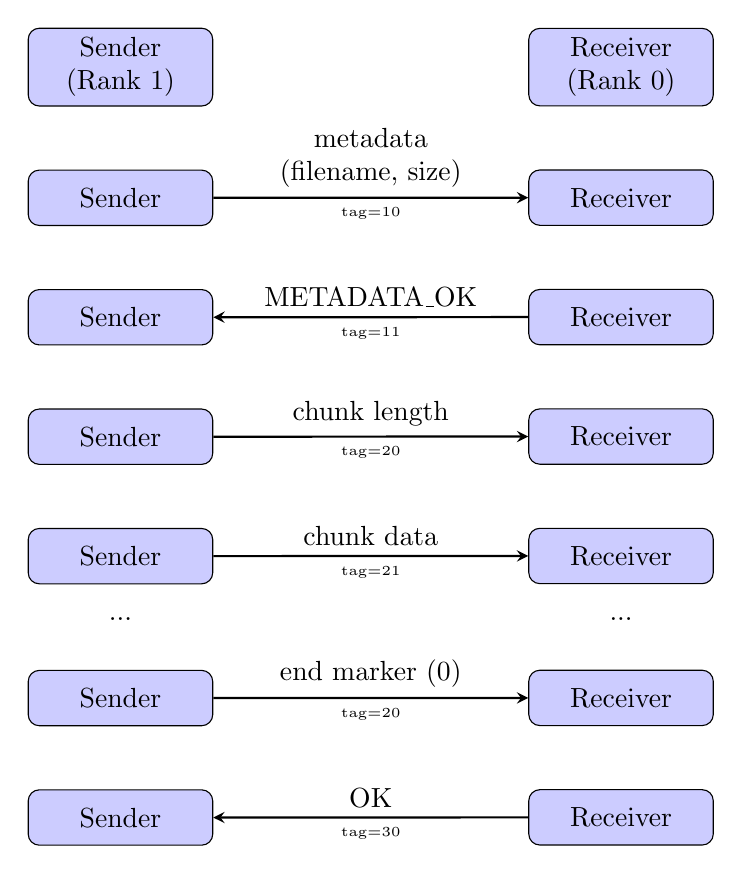
\begin{tikzpicture}[node distance=2.5cm, auto]
    % Styles
    \tikzstyle{block} = [rectangle, draw, fill=blue!20, text width=6em, text centered, rounded corners, minimum height=2em]
    \tikzstyle{arrow} = [thick,->,>=stealth]
    
    % Nodes - Sender side (Rank 1)
    \node [block] (sender1) {Sender\\(Rank 1)};
    \node [block, right=4cm of sender1] (receiver1) {Receiver\\(Rank 0)};
    
    % Step 1: Send metadata
    \node [block, below=0.8cm of sender1] (sender2) {Sender};
    \node [block, below=0.8cm of receiver1] (receiver2) {Receiver};
    \draw[arrow] (sender2.east) -- node[above, text width=3.5cm, align=center] {metadata\\ (filename, size)} node[below, font=\tiny] {tag=10} (receiver2.west);
    
    % Step 2: ACK metadata
    \node [block, below=0.8cm of sender2] (sender3) {Sender};
    \node [block, below=0.8cm of receiver2] (receiver3) {Receiver};
    \draw[arrow] (receiver3.west) -- node[above] {METADATA\_OK} node[below, font=\tiny] {tag=11} (sender3.east);
    
    % Step 3: Send chunk length
    \node [block, below=0.8cm of sender3] (sender4) {Sender};
    \node [block, below=0.8cm of receiver3] (receiver4) {Receiver};
    \draw[arrow] (sender4.east) -- node[above] {chunk length} node[below, font=\tiny] {tag=20} (receiver4.west);
    
    % Step 4: Send chunk data
    \node [block, below=0.8cm of sender4] (sender5) {Sender};
    \node [block, below=0.8cm of receiver4] (receiver5) {Receiver};
    \draw[arrow] (sender5.east) -- node[above] {chunk data} node[below, font=\tiny] {tag=21} (receiver5.west);
    
    % Step 5: Repeat (indicated by dots)
    \node [below=0.3cm of sender5] (dots1) {...};
    \node [below=0.3cm of receiver5] (dots2) {...};
    
    % Step 6: End marker
    \node [block, below=0.5cm of dots1] (sender6) {Sender};
    \node [block, below=0.5cm of dots2] (receiver6) {Receiver};
    \draw[arrow] (sender6.east) -- node[above] {end marker (0)} node[below, font=\tiny] {tag=20} (receiver6.west);
    
    % Step 7: Final ACK
    \node [block, below=0.8cm of sender6] (sender7) {Sender};
    \node [block, below=0.8cm of receiver6] (receiver7) {Receiver};
    \draw[arrow] (receiver7.west) -- node[above] {OK} node[below, font=\tiny] {tag=30} (sender7.east);
    
\end{tikzpicture}
\caption{MPI File Transfer Protocol Sequence}
\label{fig:mpi-protocol}
\end{figure}

\subsection{Process Roles}

\begin{itemize}
    \item \textbf{Rank 0 (Receiver)}: Acts as the file receiver, similar to a server in client-server architecture
    \item \textbf{Rank 1 (Sender)}: Acts as the file sender, similar to a client
\end{itemize}

\subsection{Communication Protocol}

The file transfer follows this sequence:

\begin{enumerate}
    \item \textbf{Initialization}: Both processes start via \texttt{mpiexec -n 2}
    \item \textbf{Metadata Exchange}: Sender sends filename and file size (tag=10)
    \item \textbf{Metadata Acknowledgment}: Receiver confirms ready to receive (tag=11)
    \item \textbf{Chunked Data Transfer}: 
    \begin{itemize}
        \item Sender sends chunk length (tag=20), then chunk data (tag=21)
        \item Repeated until entire file is transferred
        \item Uses 4096-byte chunks for efficiency
    \end{itemize}
    \item \textbf{End Marker}: Sender sends 0 as chunk length to signal completion (tag=20)
    \item \textbf{Final Acknowledgment}: Receiver verifies file and sends OK (tag=30)
\end{enumerate}

\subsection{Message Tags}

MPI tags distinguish different types of messages:
\begin{itemize}
    \item Tag 10: Metadata (filename, size)
    \item Tag 11: Metadata acknowledgment
    \item Tag 20: Chunk length / End marker
    \item Tag 21: Chunk data
    \item Tag 30: Final acknowledgment
\end{itemize}

\section{System Organization}

The system is organized as a single Python program that behaves differently based on its MPI rank.

\begin{figure}[h]
\centering
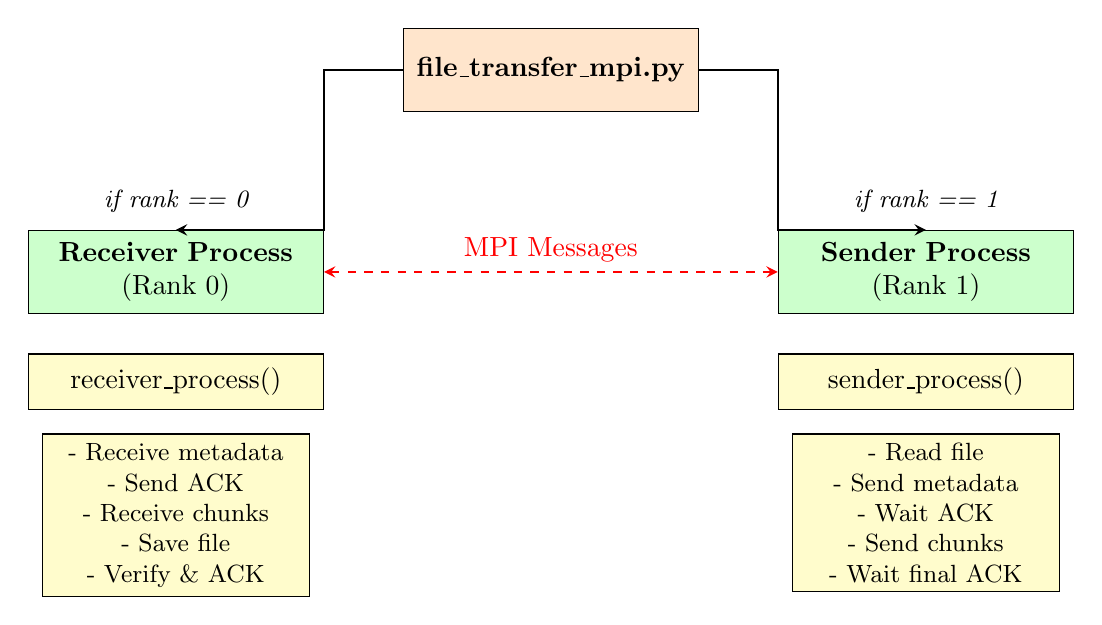
\begin{tikzpicture}[node distance=3cm, auto]
    \tikzstyle{component} = [rectangle, draw, fill=green!20, text width=10em, text centered, minimum height=3em]
    \tikzstyle{function} = [rectangle, draw, fill=yellow!20, text width=10em, text centered, minimum height=2em]
    
    % Main program
    \node [component, fill=orange!20] (main) {\textbf{file\_transfer\_mpi.py}};
    
    % Rank 0 path
    \node [component, below left=1.5cm and 1cm of main] (receiver) {\textbf{Receiver Process}\\ (Rank 0)};
    \node [function, below=0.5cm of receiver] (recv_func) {receiver\_process()};
    \node [function, below=0.3cm of recv_func, text width=9em, font=\small] (recv_steps) {
        - Receive metadata\\
        - Send ACK\\
        - Receive chunks\\
        - Save file\\
        - Verify \& ACK
    };
    
    % Rank 1 path
    \node [component, below right=1.5cm and 1cm of main] (sender) {\textbf{Sender Process}\\ (Rank 1)};
    \node [function, below=0.5cm of sender] (send_func) {sender\_process()};
    \node [function, below=0.3cm of send_func, text width=9em, font=\small] (send_steps) {
        - Read file\\
        - Send metadata\\
        - Wait ACK\\
        - Send chunks\\
        - Wait final ACK
    };
    
    % Connections
    \draw[thick,->,>=stealth] (main.west) -- +(-1,0) |- (receiver.north);
    \draw[thick,->,>=stealth] (main.east) -- +(1,0) |- (sender.north);
    
    % MPI Communication
    \draw[thick,<->,>=stealth,dashed,red] (receiver.east) -- node[above] {MPI Messages} (sender.west);
    
    % Labels
    \node[above=0.1cm of receiver, font=\small\itshape] {if rank == 0};
    \node[above=0.1cm of sender, font=\small\itshape] {if rank == 1};
    
\end{tikzpicture}
\caption{System Architecture and Process Flow}
\label{fig:architecture}
\end{figure}



\subsection{Component Description}

\textbf{Main Program (file\_transfer\_mpi.py):}
\begin{itemize}
    \item Single program with dual behavior based on MPI rank
    \item Initializes MPI environment
    \item Routes execution to sender or receiver function
    \item Handles command-line arguments and error checking
\end{itemize}

\textbf{Sender Function (sender\_process):}
\begin{itemize}
    \item Validates file existence
    \item Sends metadata dictionary via \texttt{comm.send()}
    \item Reads file in 4096-byte chunks
    \item Converts chunks to NumPy arrays for MPI transfer
    \item Uses \texttt{comm.Send()} for efficient binary data transfer
    \item Tracks and displays progress
\end{itemize}

\textbf{Receiver Function (receiver\_process):}
\begin{itemize}
    \item Receives metadata via \texttt{comm.recv()}
    \item Creates output directory if needed
    \item Receives chunks using \texttt{comm.Recv()}
    \item Writes chunks to file incrementally
    \item Verifies file integrity by comparing sizes
    \item Sends appropriate acknowledgment
\end{itemize}

\section{Implementation}

\subsection{MPI Initialization}

The program begins by initializing the MPI environment:

\begin{lstlisting}[caption=MPI Environment Setup]
from mpi4py import MPI
import numpy as np

# Get MPI communicator
comm = MPI.COMM_WORLD
rank = comm.Get_rank()  # Process ID (0 or 1)
size = comm.Get_size()  # Total processes (should be 2)

# Define roles
RECEIVER_RANK = 0
SENDER_RANK = 1
CHUNK_SIZE = 4096
\end{lstlisting}

\subsection{Metadata Exchange}

The sender transmits file metadata using Python object communication:

\begin{lstlisting}[caption=Sending Metadata (Rank 1)]
# Prepare metadata dictionary
metadata = {
    'filename': os.path.basename(filename),
    'filesize': os.path.getsize(filename)
}

# Send to receiver (uses pickle internally)
comm.send(metadata, dest=RECEIVER_RANK, tag=10)

# Wait for acknowledgment
ack = comm.recv(source=RECEIVER_RANK, tag=11)
\end{lstlisting}

\begin{lstlisting}[caption=Receiving Metadata (Rank 0)]
# Receive metadata
metadata = comm.recv(source=SENDER_RANK, tag=10)
filename = metadata['filename']
filesize = metadata['filesize']

# Send acknowledgment
comm.send("METADATA_OK", dest=SENDER_RANK, tag=11)
\end{lstlisting}

\subsection{File Data Transfer}

File data is transferred in chunks using NumPy arrays for efficiency:

\begin{lstlisting}[caption=Sending File Data (Rank 1)]
bytes_sent = 0
with open(filename, 'rb') as f:
    while bytes_sent < filesize:
        # Read chunk from file
        chunk_data = f.read(CHUNK_SIZE)
        if not chunk_data:
            break
        
        # Convert to numpy array
        chunk_array = np.frombuffer(chunk_data, dtype=np.uint8)
        chunk_length = len(chunk_array)
        
        # Send chunk length (small int)
        comm.send(chunk_length, dest=RECEIVER_RANK, tag=20)
        
        # Send chunk data (numpy array, efficient)
        comm.Send(chunk_array, dest=RECEIVER_RANK, tag=21)
        
        bytes_sent += chunk_length

# Send end marker
comm.send(0, dest=RECEIVER_RANK, tag=20)
\end{lstlisting}

\begin{lstlisting}[caption=Receiving File Data (Rank 0)]
bytes_received = 0
with open(filepath, 'wb') as f:
    while bytes_received < filesize:
        # Receive chunk length
        chunk_length = comm.recv(source=SENDER_RANK, tag=20)
        
        # Check for end marker
        if chunk_length == 0:
            break
        
        # Prepare buffer for receiving
        chunk_array = np.empty(chunk_length, dtype=np.uint8)
        
        # Receive chunk data
        comm.Recv(chunk_array, source=SENDER_RANK, tag=21)
        
        # Write to file
        f.write(chunk_array.tobytes())
        bytes_received += chunk_length
\end{lstlisting}

\subsection{File Verification}

After transfer, the receiver verifies file integrity:

\begin{lstlisting}[caption=File Verification and Final Acknowledgment]
# Check actual file size
actual_size = os.path.getsize(filepath)

if actual_size == filesize:
    print(f"File integrity verified")
    comm.send("OK", dest=SENDER_RANK, tag=30)
else:
    print(f"Size mismatch!")
    comm.send("SIZE_MISMATCH", dest=SENDER_RANK, tag=30)
\end{lstlisting}

\section{How to Design the MPI Service}

\subsection{Key Design Decisions}

\textbf{1. SPMD Architecture}
\begin{itemize}
    \item Single program simplifies development and deployment
    \item Rank-based branching determines behavior
    \item All processes start simultaneously
\end{itemize}

\textbf{2. Dual Communication Modes}
\begin{itemize}
    \item \texttt{send()}/\texttt{recv()} for Python objects (metadata, acknowledgments)
    \item \texttt{Send()}/\texttt{Recv()} for NumPy arrays (file data)
    \item This hybrid approach balances convenience and performance
\end{itemize}

\textbf{3. Tag-Based Message Typing}
\begin{itemize}
    \item Different tags prevent message confusion
    \item Enables out-of-order processing if needed
    \item Clear protocol definition
\end{itemize}

\textbf{4. Chunked Transfer with Progress Tracking}
\begin{itemize}
    \item 4096-byte chunks prevent memory overflow
    \item Enables real-time progress display
    \item Allows for potential pause/resume functionality
\end{itemize}

\textbf{5. Multi-Level Acknowledgment}
\begin{itemize}
    \item Metadata ACK ensures receiver is ready
    \item Final ACK confirms successful transfer
    \item Provides reliability without complex error handling
\end{itemize}

\subsection{Advantages Over TCP}

\begin{tabular}{|p{4cm}|p{5cm}|p{5cm}|}
\hline
\textbf{Aspect} & \textbf{TCP (Practice 1)} & \textbf{MPI (Practice 3)} \\
\hline
Setup & Separate server/client programs & Single program, multiple ranks \\
\hline
Connection & Manual socket creation & MPI handles communication \\
\hline
Addressing & IP address:Port & Process rank \\
\hline
Message Types & Raw bytes only & Objects and arrays \\
\hline
Scalability & 1-to-1 only & Easily extends to N processes \\
\hline
Environment & General purpose & Optimized for HPC \\
\hline
\end{tabular}

\section{How to Organize the System}

\subsection{Process Organization}

The system uses a simple 2-process model:

\begin{figure}[h]
\centering
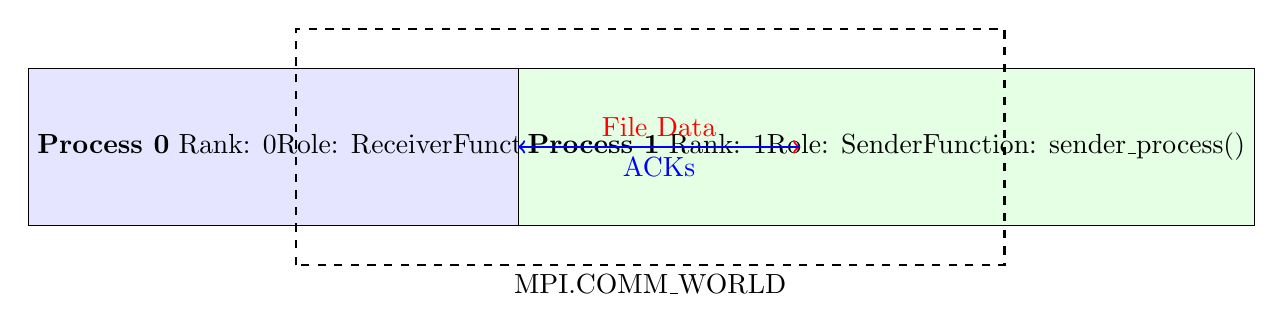
\begin{tikzpicture}
    % Two processes
    \node[draw, rectangle, minimum width=3cm, minimum height=2cm, fill=blue!10] (p0) at (0,0) {
        \textbf{Process 0}\\[0.5em]
        Rank: 0\\
        Role: Receiver\\
        Function: receiver\_process()
    };
    
    \node[draw, rectangle, minimum width=3cm, minimum height=2cm, fill=green!10] (p1) at (6,0) {
        \textbf{Process 1}\\[0.5em]
        Rank: 1\\
        Role: Sender\\
        Function: sender\_process()
    };
    
    % Communication
    \draw[->,thick,red] (p1.west) -- node[above] {File Data} (p0.east);
    \draw[->,thick,blue] (p0.east) -- node[below] {ACKs} (p1.west);
    
    % MPI Communicator
    \draw[dashed,thick] (-1.5,-1.5) rectangle (7.5,1.5);
    \node[below] at (3,-1.5) {MPI.COMM\_WORLD};
\end{tikzpicture}
\caption{Process Organization in MPI File Transfer}
\end{figure}

\subsection{Data Flow}

\begin{enumerate}
    \item \textbf{Input}: Sender reads file from filesystem
    \item \textbf{Processing}: File is chunked and converted to NumPy arrays
    \item \textbf{Communication}: Chunks transmitted via MPI point-to-point messages
    \item \textbf{Output}: Receiver writes chunks to disk in \texttt{received\_files/}
\end{enumerate}

\subsection{Error Handling}

\begin{itemize}
    \item File not found: Check before sending
    \item Wrong number of processes: Validate at startup
    \item Size mismatch: Verify after transfer
    \item Exceptions: Try-catch blocks with error messages
\end{itemize}

\section{Code Implementation Details}

\subsection{Running the Program}

\begin{lstlisting}[language=bash, caption=Execution Command]
# Basic usage
mpiexec -n 2 python file_transfer_mpi.py test_file.txt

# The above command:
# -n 2: Start 2 MPI processes
# Rank 0: Acts as receiver
# Rank 1: Reads and sends test_file.txt
\end{lstlisting}

\subsection{Key Code Structure}

\begin{lstlisting}[caption=Main Function Structure]
def main():
    # Check process count
    if size != 2:
        print("Error: Requires exactly 2 processes")
        return
    
    # Branch based on rank
    if rank == SENDER_RANK:
        # Get filename from command line
        filename = sys.argv[1]
        sender_process(filename)
    elif rank == RECEIVER_RANK:
        receiver_process()
\end{lstlisting}



\section{Testing and Verification}

The system was tested with:

\subsection{Test Cases}
\begin{itemize}
    \item Small text files ($<$ 1KB) - test\_file.txt
    \item Medium files (1-10 MB) - Various documents
    \item Binary files - Images, PDFs
\end{itemize}

\subsection{Verification Methods}
\begin{enumerate}
    \item File size comparison (automatic in code)
    \item Content verification using diff tools
    \item Multiple consecutive transfers
    \item Progress display accuracy
\end{enumerate}

All tests completed successfully with files received intact.

\section{Conclusion}

This practice successfully implements an MPI-based file transfer system using mpi4py. The implementation demonstrates understanding of:

\begin{itemize}
    \item MPI fundamentals and SPMD architecture
    \item Point-to-point communication using send/recv
    \item Efficient binary data transfer with NumPy arrays
    \item Process synchronization and acknowledgment protocols
    \item Tag-based message differentiation
    \item Chunked data transfer for large files
\end{itemize}

\subsection{Key Differences from TCP Implementation}

The MPI approach offers several advantages:
\begin{itemize}
    \item \textbf{Simpler deployment}: Single program instead of separate client/server
    \item \textbf{Better abstraction}: MPI handles low-level communication details
    \item \textbf{Scalability}: Easy to extend to multiple senders/receivers
    \item \textbf{Performance}: Optimized for HPC environments
    \item \textbf{Portability}: Standard interface across platforms
\end{itemize}

\subsection{Lessons Learned}

\begin{enumerate}
    \item MPI's SPMD model requires different thinking than client-server
    \item Using both \texttt{send()} and \texttt{Send()} leverages Python and performance
    \item NumPy integration is crucial for efficient binary data transfer
    \item Message tags are essential for protocol clarity
    \item MPI is particularly well-suited for parallel computing scenarios
\end{enumerate}

\subsection{Future Enhancements}

Possible extensions include:
\begin{itemize}
    \item Multi-file transfer in a single session
    \item Compression before transfer
    \item Collective operations for broadcast to multiple receivers
    \item Non-blocking (asynchronous) communication
    \item Integration with parallel file systems
\end{itemize}

This MPI file transfer system provides a solid foundation for understanding distributed communication in high-performance computing environments.

\end{document}
